\documentclass[a4paper]{article}

%% Language and font encodings
\usepackage[english]{babel}
\usepackage[utf8x]{inputenc}
\usepackage[T1]{fontenc}

%% Sets page size and margins
\usepackage[a4paper,top=3cm,bottom=2cm,left=3cm,right=3cm,marginparwidth=1.75cm]{geometry}

%% Useful packages
\usepackage{amsmath}
\usepackage{graphicx}
\usepackage[colorinlistoftodos]{todonotes}
\usepackage[colorlinks=true, allcolors=blue]{hyperref}
\usepackage{float}


\title{Benchmarking P2C for HPC using NPB}
\author{Joseph Anthony C. Hermocilla}

\begin{document}
\maketitle

\begin{abstract}
We report some benchmarking results of the Peak-Two Cloud(P2C) for High-Performance Computing(HPC) using the NAS Parallel Benchmarks(NPB).
\end{abstract}

\section{Introduction}

In order to evaluate the performance of the P2C\cite{hermocilla-p2c-ncite2014} for HPC, NPB\footnote{https://www.nas.nasa.gov/publications/npb.html} version 3.3.1 was run on a 16-node MPI cluster provisioned using vcluster\footnote{http://srg.ics.uplb.edu.ph/projects/peak-two-cloud/peak-two-cloud-resources/deployinganmpiclusterusingvcluster}.

NPB consists of a set of programs that implements different computational approaches associated with Computational Fluid Dynamics(CFD). These programs represent the types of applications that are run in supercomputers and HPC clusters. In running the benchmark, classes A and B were used for each program. Different classes have different problem sizes and parameters which result to different measurements.

The programs were run using 1, 2, 4, 8, and 16 nodes. The completion times were recorded and plotted. 
The figure below (insert figure here) shows the hosts where the VMs used in the cluster were instantiated. 


\section{Results}

The following subsections show the completion time for each program in NPB tested using different number of nodes. Ideally, the completion time of the programs should decrease as the number of nodes is increased. However, the results show some fluctuations for some programs. 

\subsection{Conjugate Gradient}

Performs irregular memory access and communication.

\begin{figure}[H]
\centering
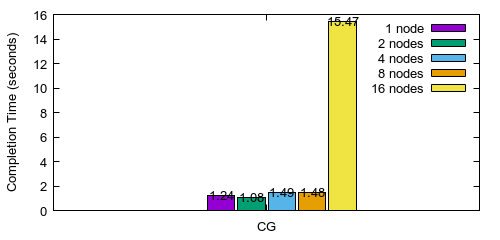
\includegraphics[width=0.8\textwidth]{figures/CGvA.png}
\caption{\label{fig:CGvA}CG, Class A}
\end{figure}

\begin{figure}[H]
\centering
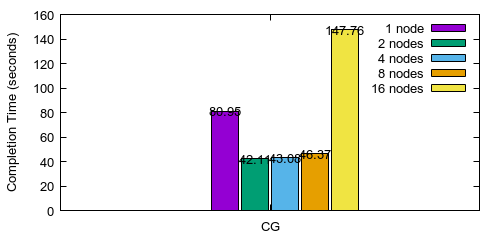
\includegraphics[width=0.8\textwidth]{figures/CGvB.png}
\caption{\label{fig:CGvB}CG, Class B}
\end{figure}

\subsection{Embarassingly Parallel}

An application with very minimal communication and synchronization to complete a task.

\begin{figure}[H]
\centering
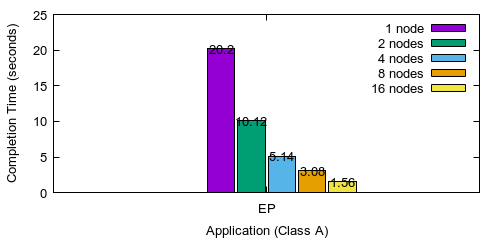
\includegraphics[width=0.8\textwidth]{figures/EPvA.png}
\caption{\label{fig:EPvA}EP, Class A}
\end{figure}

\begin{figure}[H]
\centering
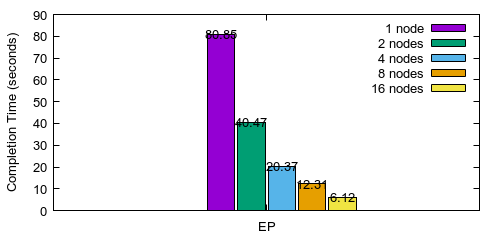
\includegraphics[width=0.8\textwidth]{figures/EPvB.png}
\caption{\label{fig:EPvB}EP, Class B}
\end{figure}


\subsection{Fourier Transform}
Performs all-to-all communication.


\begin{figure}[H]
\centering
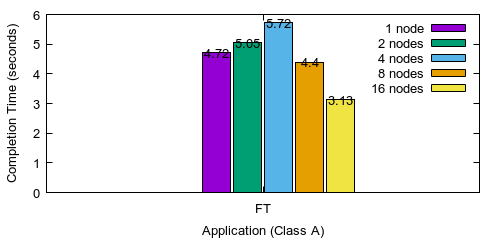
\includegraphics[width=0.8\textwidth]{figures/FTvA.png}
\caption{\label{fig:FTvA}FT, Class A}
\end{figure}

\begin{figure}[H]
\centering
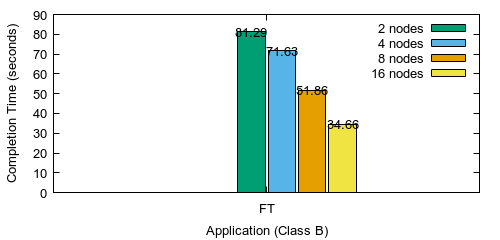
\includegraphics[width=0.8\textwidth]{figures/FTvB.png}
\caption{\label{fig:FTvB}FT, Class B}
\end{figure}

\subsection{Integer Sort}
Performs random memory access.


\begin{figure}[H]
\centering
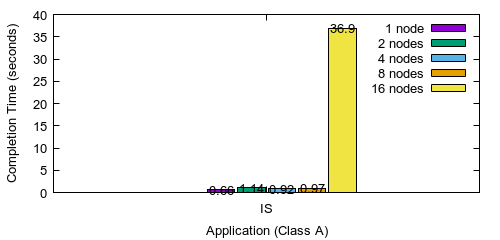
\includegraphics[width=0.8\textwidth]{figures/ISvA.png}
\caption{\label{fig:ISvA}IS, Class A}
\end{figure}

\begin{figure}[H]
\centering
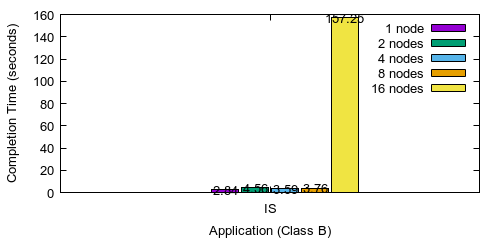
\includegraphics[width=0.8\textwidth]{figures/ISvB.png}
\caption{\label{fig:ISvB}IS, Class B}
\end{figure}

\subsection{Lower-Upper Gauss-Seidel Solver}

A pseudo application that solves a system of linear equations.

\begin{figure}[H]
\centering
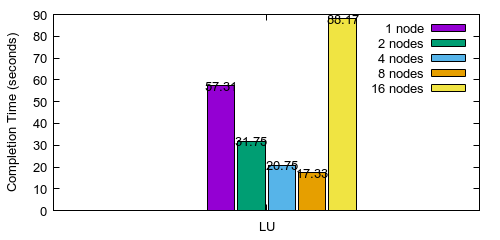
\includegraphics[width=0.8\textwidth]{figures/LUvA.png}
\caption{\label{fig:LUvA}LU, Class A}
\end{figure}

\begin{figure}[H]
\centering
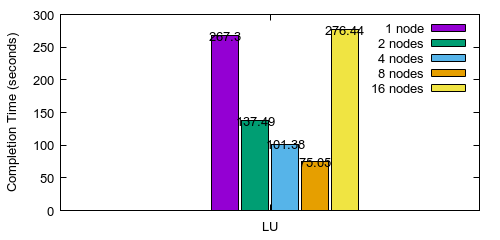
\includegraphics[width=0.8\textwidth]{figures/LUvB.png}
\caption{\label{fig:LUvB}LU, Class B}
\end{figure}

\subsection{Multi-Grid}

Solves differential equations using long- and short-distance communication and is memory intensive.

\begin{figure}[H]
\centering
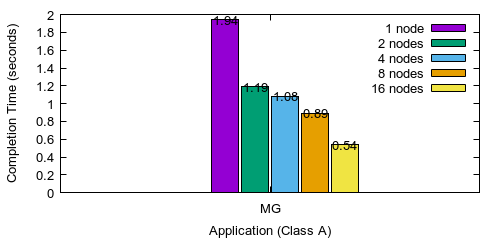
\includegraphics[width=0.8\textwidth]{figures/MGvA.png}
\caption{\label{fig:MGvA}MG, Class A}
\end{figure}

\begin{figure}[H]
\centering
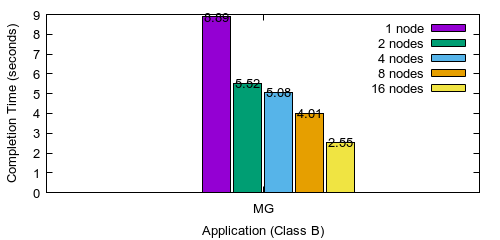
\includegraphics[width=0.8\textwidth]{figures/MGvB.png}
\caption{\label{fig:MGvB}MG, Class B}
\end{figure}

\bibliographystyle{abbrv}
\bibliography{p2c-benchmark}

\end{document}